\chapter{Background} In the domain of High-Performance
Computing (HPC) and data center networks, the coordination of numerous hardware
components is crucial for them to function as a unified system. This
coordination happens through an interconnection network, which serves as the
backbone for communication among these components. Thousands of hardware pieces
collaborate over this interconnection network to ensure smooth operation. The
effectiveness of this interconnect relies on various design choices, such as the
topology used to connect physical components, the routing scheme to select
communication paths, and managing network traffic loads along these paths and
links.  In this chapter, I provide essential background information on topology,
routing and Software Defined Networks (SDN). By covering these fundamental
concepts, readers will gain insight into how hardware components interact and
how interconnect designs can be optimized for better performance within HPC and
data center environments

\section{Topology} The interconnect network is usually shown as a graph, where
each point (vertex) represents a piece of hardware like a server or a switch,
and each line (edge) represents a connection between them. I usually refer to
servers as processing elements, and switches or routers as forwarding elements.
When two points are directly connected by a line, I say they are neighbors. The
number of connections a point has is called its nodal degree. The distance
between two points is how many connections (or hops) it takes to get from one to
the other. The diameter of a network is the longest distance between any two
points.  Splitting the network into two equal halves is called a bisection, and
the bandwidth of this split is how much data can flow between the two halves
without slowing down. The bisection bandwidth is the lowest possible bandwidth
among all possible splits.  If the bandwidth is low, it can slow down traffic.
For networks used in HPC and data centers, I want a low diameter and high
bisection bandwidth to perform well at scale. I also aim for a low nodal degree
to keep costs down and avoid complex designs.  To meet these challenges,
different types of topologies are used. In data centers, one of the most
commonly utilized interconnection topologies is the fat-tree. This design has
gained popularity due to its ability to efficiently provide a high throughput
and low latency for communication. For bigger systems, like exascale
supercomputers, the Dragonfly topology has been gaining popularity recently.
It's designed to be scalable and cost-effective on a large scale. As technology
evolves, new topologies will likely be developed to meet the demands of future
interconnects.

\subsection{Fat-Tree} Fat-tree topology represents a robust architecture for
high-performance computing environments, characterized by its hierarchical
structure and abundant bandwidth allocation ~\cite{leiserson1985fat}. In this topology, switches and
compute nodes are organized into a tree-like structure, with bandwidth
increasing as one ascends toward the root of the tree.  Hierarchy and Switch
Types: In a typical fat-tree setup, such as the 3-level full bisection bandwidth
fat-tree, switches are classified into three categories: 

\begin{itemize} 
\item \textbf{Core Switches :} These switches reside at the highest layer and serve to interconnect different pods.
\item \textbf{Aggregate Switches :} Positioned between the core and leaf switches, aggregate switches link to the leaf switches within a pod, forming a cohesive unit.
\item \textbf{Leaf Switches :} Located at the bottom layer, leaf switches interface directly with the compute nodes, facilitating communication within the pod.
\end{itemize} 

\begin{figure}[h]
  \centering
  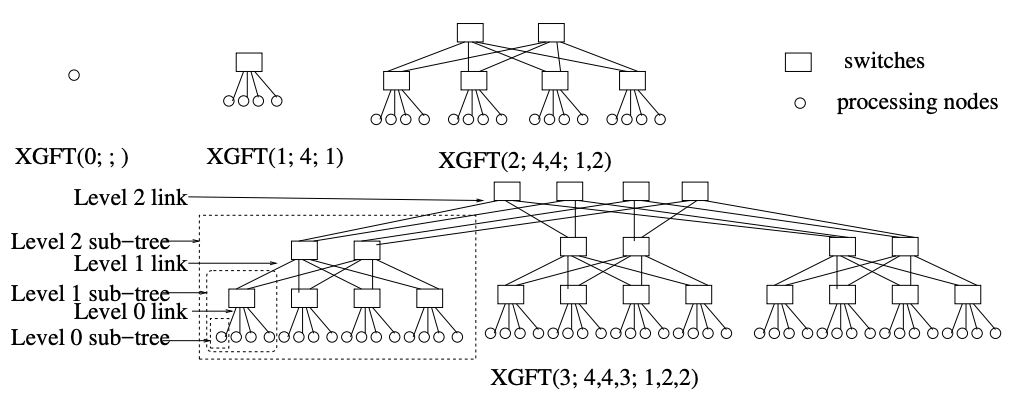
\includegraphics[width=0.8\columnwidth]{./figs/xgft.png}
  \caption{A fat-tree represented in XGFT.}
  \label{fig:fat-treexgft}
\end{figure}

Fat-tree topology ensures that the bandwidth within a level
remains consistent, if not increasing, as one moves toward higher levels\cite{leiserson1985fat, jain2017predicting}.  A
full bisection bandwidth fat-tree is a type of network configuration designed to
ensure that every node on one half of the network can communicate with every
other node in the other half of the network without creating bottlenecks. In
this setup, the bandwidth between any two points in the network is maximized,
which helps to prevent congestion and ensures smooth communication. To ensure
full bisection bandwidth, more network resources are allocated, which increases
the cost.  One method used to reduce the cost of building a fat-tree network is
tapering. Tapering involves connecting more devices to each switch at the lower
levels of the network, known as leaf switches. While this may decrease the total
bandwidth available at higher levels, it also reduces the number of switches and
cables needed to connect the same number of devices compared to a full fat-tree
configuration.  Full bisection bandwidth fat-tree networks can be described
using two key parameters: 'm' and 'n'. The parameter 'm' signifies the degree of
all internal nodes, which must be divisible by 2. Meanwhile, 'n' denotes the
number of levels of internal nodes, resulting in a fat-tree with n + 1 levels in
total\cite{leiserson1985fat}.  To economize network costs, tapering strategies can be implemented,
allowing for more nodes to be connected per leaf switch. For
comprehensive representation and analysis of any fat-tree topologies, Ohring
introduced extended generalized fat tree (XGFT) representations\cite{ohring1995generalized}. These
representations provide a structured method for describing fat-tree
configurations, aiding in both design and analysis processes. The XGFT notation,
capable of representing various fat-tree variations, specifies a fat tree of
height 'h', comprising h + 1 levels of nodes. Each level is labeled from 0 to h,
starting with processing nodes at level 0. Moreover, each node at level 'i' 
\begin{comment}
(0 \leq i \leq h - 1) 
\end{comment}
has 'wi' parents, while each node at level 'i' 
\begin{comment}
(1 \leq i \leq h) 
\end{comment}
has 'mi-1'
children. This notation is exemplified by the recursive construction of XGFT(3;
4, 4, 3; 1, 2, 2), where 'h' equals 3, 'm0' equals 4, 'm1' equals 4, 'm2' equals
3, 'w0' equals 1, 'w1' equals 2, and 'w2' equals 2.  

\subsection{Dragonfly} The Dragonfly topology stands out as a cost-effective
solution for building expansive interconnection networks \cite{kim2008technology}. This design is
characterized by its two-layer structure, exemplified in Figure \ref{fig:dfly}. Initially
proposed by Kim et al. \cite{kim2008technology}, the Dragonfly topology employs a multi-level dense
configuration, primarily leveraging high-radix routers.  In its basic form, a
Dragonfly network comprises interconnected routers forming groups, each
resembling a virtual router with a notably high radix [8]. These groups are then
interconnected through an inter-group topology. In a practical scenario, such as
the one illustrated in Figure ~\ref{fig:dfly}, each group typically encompasses 4 switches,
culminating in a total of 9 groups within the network.  There are variations of
Dragonfly topology, including Canonical Dragonfly, Hamming Dragonfly, and
Dragonfly Plus, which utilize various intra-group connectivity patterns \cite{hastings2015comparing}.
However, all implementations of Dragonfly topology feature all-to-all
connectivity between groups. At the inter-group level, Dragonfly networks
consistently adopt a fully connected topology.  A crucial aspect of the
Dragonfly topology revolves around three key parameters: the number of compute
nodes in each switch (p), the intra-group links per switch (a), and the
inter-group links per switch (h) ~\cite{kim2008technology}. 

\begin{figure}[h]
  \centering
  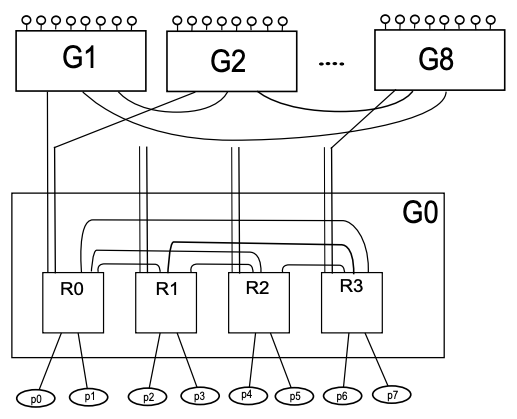
\includegraphics[width=0.8\columnwidth]{figs/dfly.png}
  \caption{Dragonfly architecture with 9 groups and 4 routers per group}
  \label{fig:dfly}
\end{figure}


The Dragonfly network comprises a total of
g groups, g × a routers, and g × a × p compute nodes, where 'g' represents the
number of groups, 'a' signifies the intra-group links per switch, and 'p'
denotes the compute nodes per switch. Each group has a × h global links, with
'h' representing the inter-group links per switch. Notably, the maximum size
Dragonfly configuration is characterized by g = a × h + 1 groups.  A balanced
Dragonfly configuration typically necessitates a = 2p = 2h, ensuring efficient
load distribution across the network.  Several prominent supercomputer
architectures, such as the Cray Cascade architecture and the Cray Slingshot
network, have embraced variations of the Dragonfly topology \cite{faanes2012cray, de2020depth}. These
implementations have found their way into current supercomputers like Titan \cite{titan} and
Trinity \cite{archer2015trinity}, as well as future exascale computing designs.  In summary, the
Dragonfly topology, with its versatile structure and efficient utilization of
high-radix routers, presents a compelling solution for constructing large-scale
interconnection networks, offering both cost-effectiveness and scalability.

\section{Routing}

Efficient routing plays a critical role in optimizing network flow by determining the most effective paths for data transmission. Routing in general determines how data packets, which are units of data transmitted over a network, travel from a starting point to an endpoint within a network. Each data packet contains information such as the source address, destination address, and the actual data being transmitted. These packets are sent from a source node to a destination node, with each node being connected to a switch. The source switch connects to the source server, while the destination switch connects to the destination server. It involves mapping network flows to specific paths for data transmission, a process influenced by the network's underlying topology. The efficiency of routing directly impacts the performance of applications in HPC and data center systems, making it a crucial aspect of interconnect modeling. Different routing schemes cater to various interconnect designs, with four common approaches being deterministic routing, adaptive routing, source routing, and hop-by-hop routing. Deterministic routing precomputes paths for each source-destination pair, with packets consistently sent along these predetermined paths. Adaptive routing dynamically selects paths based on the current network state, allowing for real-time adjustments to optimize performance. Source routing involves the source node determining the complete path for each packet and embedding this routing information within the packet header, while hop-by-hop routing allows each intermediate node along the path to independently make routing decisions based on local routing tables or forwarding rules. These routing strategies play a vital role in ensuring efficient data transmission in HPC and data center environments.

\subsection{Routing in Fat-tree}
Routing strategies within fat-tree networks can be categorized as either oblivious or adaptive to network communication traffic. In fat-tree networks, oblivious routing algorithms consistently select the same nearest common ancestor (NCA) for all communication between a given source-destination pair. These routing paths can be pre-computed and stored in forwarding tables or calculated dynamically based on simple formulas using source and destination labels. Two common oblivious routing schemes in fat-tree networks are Source-mod-k (S-mod-k) and Destination-mod-k (D-mod-k). Both S-mod-k and D-mod-k are considered equivalent in terms of conceptual design and performance. However, the D-mod-k algorithm may exhibit poor performance for both average and worst-case permutation traffic patterns. In contrast, adaptive routing algorithms dynamically select paths based on the current network state, such as link congestion or available bandwidth, to optimize performance in real-time. In adaptive routing within fat-tree networks, the routing strategy dynamically selects paths based on the current network state, such as link congestion or available bandwidth, to optimize performance in real-time. During the upward direction toward the nearest common ancestor (NCA) for both the source and destination routers, adaptive routing algorithms prioritize forwarding packets to the least congested port available. This approach helps to alleviate congestion and optimize the utilization of network resources by steering traffic along paths with ample capacity. Once the packet reaches the NCA, which acts as the central router for the source-destination pair, it is then directed along a unique downward path toward the destination router. By dynamically adapting routing paths based on real-time network conditions, adaptive routing enhances the efficiency and performance of fat-tree networks. Routing decisions in fat-tree networks typically focus on determining the upward paths to carry traffic for each source-destination pair.

\subsection{Routing in Dragonfly}
In a Dragonfly topology, the source node belongs to the source group, and the destination node belongs to the destination group. Traffic packets between these nodes can travel along either a minimal or a non-minimal path. Broadly speaking, the Dragonfly network has three popular routing schemes.
First, I have the Minimal Routing (MIN) scheme \cite{kim2008technology}, which directs data packets exclusively along the shortest routes between source and destination nodes. Minimal paths typically involve traversing one global link at most. MIN routing aims to minimize resource usage and is effective for traffic patterns such as random uniform traffic. Suppose I have a Dragonfly network topology where a source node 'S' in group A needs to communicate with a destination node 'D' in group B. In MIN routing, the data packet would follow the shortest path, traversing one global link at most. For example, the packet might first travel from 'S' to a switch in group B via a global link, then to 'D' within group B.
Second, I have Valiant Load-Balanced Routing (VLB) \cite{kim2008technology, kaplan2017unveiling}, which spreads non-uniform traffic evenly across available links to mitigate congestion. It involves routing from the source to an intermediate switch, then to the destination. VLB paths are non-minimal and aim to balance traffic distribution across the network. In VLB routing, the data packet would be routed from 'S' to an intermediate switch 'I', which is not present in either source group or destination group, then to 'D'. For instance, the packet might travel from 'S' to 'I' via a global link, then from 'I' to 'D' through a global link. One of the drawbacks of VLB routing is that it increases the hop count for the transmission of data.
Finally, I have Universal Globally Adaptive Load-Balanced Routing (UGAL) \cite{kim2008technology, kaplan2017unveiling}, which dynamically selects between MIN and VLB paths based on network conditions. UGAL utilizes the buffer occupancy in the source router to estimate network congestion in real-time. This means that UGAL monitors the amount of data packets queued up or waiting to be transmitted at the source router. By assessing the level of buffer occupancy, UGAL can infer the current state of congestion within the network. If the buffer occupancy is high, indicating congestion, UGAL may opt for routing strategies that help alleviate congestion, such as selecting Valiant Load-Balanced (VLB) paths to distribute traffic more evenly across available links. It chooses a path with the smallest packet delay from a small number of candidate MIN and VLB paths. For example, if the network senses congestion on minimal paths, it might choose a VLB path for certain packets to balance the traffic load. Conversely, if the network conditions allow, it might opt for a minimal path to minimize latency.




\section{HPC Applications}
In the realm of High-Performance Computing (HPC), applications span a wide spectrum, including real-world problem-solving (a.k.a. real applications), proxy modeling (a.k.a. proxy applications), and synthetic traffic. Whether simulating climate patterns, optimizing financial portfolios, or deciphering genomic data, all HPC applications share a common iterative structure. Each iteration entails a sequence of computational tasks executed in parallel, followed by communication and synchronization steps. These iterations form the backbone of HPC workflows, where complex computations are distributed across vast computational resources. As data flows through the system, results are exchanged, aggregated, and synchronized to drive iterative refinement and convergence.

\textcolor{red}{In my work I have chosen a set of benchmarks which is represents the diverse HPC workloads, to ensure that the performance evaluation of my algorithms is comprehensive and applicable across a wide array of HPC scenarios.}
The following is a brief description of the applications I used in this work:

\begin{itemize}
\item \textbf{Random permutation}: A synthetic traffic where each node sends message to another randomly chosen node. The source destination pair is unique across the whole permutation.
\item \textbf{Stencil4d}: MPI benchmark with 8-point near-neighbor communication in a 4D virtual process grid.
\item \textbf{Subcomm3d}: MPI benchmark with all-to-all communication within subsets of processes in a 3D virtual process grid.
\item \textbf{Kripke}: 3D $S^n$ deterministic particle transport code, which runs an MPI-based parallel sweep algorithm \cite{kripke}. 
\item \textbf{Laghos}: Proxy application that solves time-dependent Euler equations with MPI-based domain decomposition \cite{laghos}.
\item \textbf{AMG}:  Parallel algebraic multigrid solver \cite{amg}.
\item \textbf{SW4lite}: Proxy application for SW4~\cite{sjogreen2018sw4}, a 3D seismic modeling code.
\item \textbf{Lammps}: LAMMPS is an acronym for Large-scale Atomic/Molecular Massively Parallel Simulator, it equations of motion for a collection of interacting particles. It partitions the simulation domain into small sub-domains to solve a problem \cite{thompson2022lammps}.
\item \textbf{Nekbone}: Solves 3D Poisson problem in rectangular geometry. The key MPI operations are matrix-matrix multiplication, inner products, nearest neighbor communicaton, MPI\_Allreduce \cite{gong2016nekbone}.
\item \textbf{MILC}: Performs four dimensional SU(3) lattice gauge theory, mainly through near-neighbour communication and MPI\_Allreduce \cite{gottlieb2001benchmarking}.
\end{itemize}

\section{Software Defined Network}
Software Defined Network(SDN) is a modern networking scheme where, the organization of network functionality is often conceptualized into three distinct layers: the data plane, the control plane, and the management plane \cite{kreutz2014software}. Each layer serves a critical role in facilitating the efficient operation and management of the network infrastructure.

\begin{figure}[h]
  \centering
  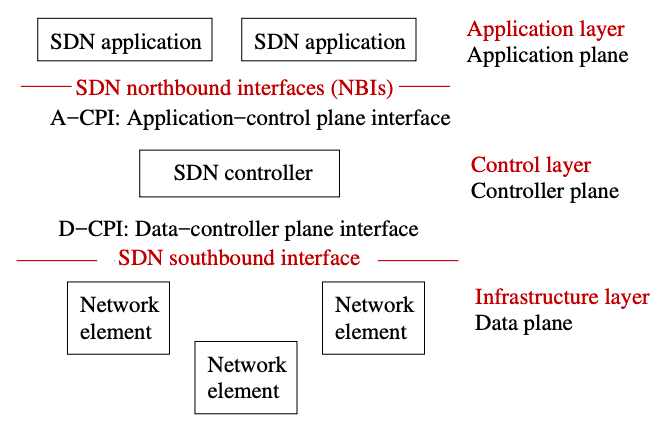
\includegraphics[width=0.8\columnwidth]{figs/sdn.png}
  \caption{SDN abstraction }
  \label{fig:sdn_abs}
%\end{multicols}
\end{figure}


\begin{itemize}
\item  \textbf{Data Plane :} The data plane, also known as the forwarding plane, is responsible for the actual transmission of data packets within the network \cite{tr2016sdn}. It consists of networking devices such as routers, switches, and other forwarding elements. These devices receive incoming packets and make forwarding decisions based on predetermined rules or protocols. The primary function of the data plane is to ensure that data packets are correctly routed to their intended destinations across the network.
\item  \textbf{Control Plane :} The control plane is tasked with managing the forwarding and routing mechanisms within the network\cite{tr2016sdn}. It determines how data packets should be forwarded based on factors such as network topology, traffic conditions, and routing policies. Traditionally, the control plane functions are embedded within the networking devices themselves, leading to a tightly coupled architecture where control and data planes operate in conjunction with each other. This tightly integrated approach has been essential for ensuring network resilience and stability, particularly in large-scale distributed networks such as the Internet.
\item \textbf{Management Plane :} The management plane oversees the overall management and configuration of the network infrastructure \cite{tr2016sdn}. It is responsible for tasks such as network monitoring, configuration management, performance optimization, and security policy enforcement. The management plane provides administrators with the tools and interfaces necessary to manage and control various aspects of the network, ensuring its reliability, security, and efficiency.
\end{itemize}

While the traditional networking architecture with tightly coupled control and data planes has been successful in ensuring network resilience, it also poses several limitations. One of the primary challenges is the complexity and rigidity of the architecture, which makes it difficult to introduce innovations and adapt to changing network requirements. Additionally, the decentralized nature of the control plane makes it challenging to achieve a holistic view of the network, hindering effective management and optimization.
To address these limitations and enable greater flexibility and agility in network management, the concept of Software-Defined Networking (SDN) has emerged as a promising approach. SDN decouples the control plane from the data plane, allowing for centralized management and programmability of the network. In an SDN architecture, the control logic is moved to a centralized entity known as the controller or Network Operating System (NOS), which maintains a global view of the network and is responsible for configuring forwarding policies.

The key components of an SDN architecture include the following:

\begin{itemize}

\item \textbf{Decoupled Data and Control Planes :} By separating the control logic from the underlying networking devices, SDN enables greater flexibility, scalability, and agility in network management. It allows administrators to dynamically adjust network behavior in response to changing traffic patterns and application requirements, leading to improved performance and resource utilization \cite{tr2016sdn, kreutz2014software}.

\item \textbf{Centralized Controller :} The centralized controller serves as the brain of the SDN architecture, maintaining a global view of the network and orchestrating the forwarding policies for all connected devices. The controller communicates with the networking devices via standardized protocols such as OpenFlow, providing a centralized point of control for the entire network \cite{tr2016sdn, kreutz2014software}.

\item \textbf{Programmable Network Behavior :} One of the key advantages of SDN is its programmability, which enables administrators to implement innovative networking services and applications through software applications running on top of the SDN controller. This programmability allows for the dynamic creation and deployment of network policies, enabling administrators to tailor the network behavior to specific application requirements and business needs \cite{tr2016sdn, kreutz2014software}.

\end{itemize}




In recent years, SDN has gained widespread acceptance and adoption in both industry and research communities. Its flexibility and programmability have led to a wide range of applications across various domains, including data centers, telecommunications, and cloud computing \cite{alalmaei2020sdn, faizian2017comparative}. 
One area of particular interest is the application of SDN in high-performance computing (HPC) environments. HPC systems often require fast and efficient communication between compute nodes to handle large-scale scientific computations and data-intensive workloads. By leveraging SDN, researchers aim to optimize routing and topologies in HPC environments, improving communication efficiency and resource utilization.

\begin{figure}[h]
  \centering
  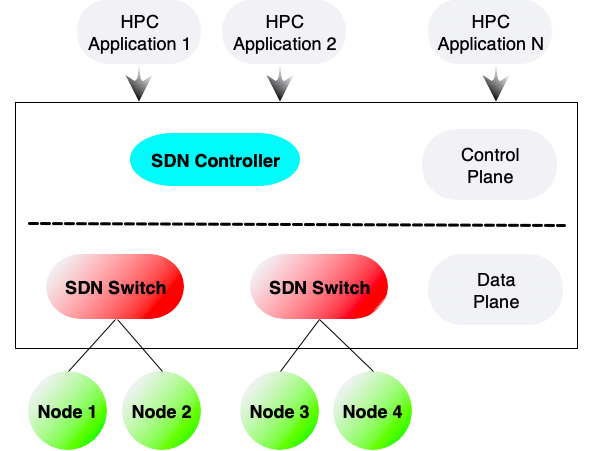
\includegraphics[width=\columnwidth]{./figs/sdn_in_hpc.png}
  \caption{SDN based HPC System (SHS)}
  \label{fig:sdn_hpc}
\end{figure}

The structure of an SDN based HPC System (SHS) is depicted in Figure~\ref{fig:sdn_hpc}.
The SDN switches perform a simple data plane functionality: packet forwarding. The
control plane is performed by the logically centralized
SDN controller (sometimes called the network operating system), which controls
the SDN switches through an interface ~\cite{benzekki2016software}.
The SDN controller provides another layer of network abstraction upon which SDN
applications can be built. When running HPC applications in an SDN based HPC system,
the applications run on the compute nodes connected to the SDN switches,
the applications use the services provided by the SDN controller to perform
communications



The remainder of this prospectus will delve into the specific challenges and opportunities associated with integrating SDN into HPC environments. It will explore novel approaches to optimizing routing, with the goal of enhancing the performance and scalability of state-of-the-art igh-performance computing (HPC) environments in the era of Software-Defined Networking.

